%%%%%%%%%%%%%%%%%%%%%%%%%%%%%%%%%%%%%%%%%%%%%%%%%%%%%%%%%%%%%%%%%%%%%%%%%%%%%%%%
%2345678901234567890123456789012345678901234567890123456789012345678901234567890
%        1         2         3         4         5         6         7         8

\documentclass[a4paper, 11.5 pt, conference]{ieeeconf}  % Comment this line out
                                                          % if you need a4paper
%\documentclass[a4paper, 10pt, conference]{ieeeconf}      % Use this line for a4
                                                          % paper

\IEEEoverridecommandlockouts                              % This command is only
                                                          % needed if you want to
                                                          % use the \thanks command
\overrideIEEEmargins
% See the \addtolength command later in the file to balance the column lengths
% on the last page of the document

% The following packages can be found on http:\\www.ctan.org
%\usepackage{graphics} % for pdf, bitmapped graphics files
%\usepackage{epsfig} % for postscript graphics files
%\usepackage{mathptmx} % assumes new font selection scheme installed
%\usepackage{times} % assumes new font selection scheme installed
%\usepackage{amsmath} % assumes amsmath package installed
%\usepackage{amssymb}  % assumes amsmath package installed

\title{\LARGE \bf
Proposal for a Course Scheduling Visualizing Software \\
 \large Object-Oriented Programming Class (ENGR-UH 2510-LAB) - Term Project
}

%\author{ \parbox{3 in}{\centering Huibert Kwakernaak*
%         \thanks{*Use the $\backslash$thanks command to put information here}\\
%         Faculty of Electrical Engineering, Mathematics and Computer Science\\
%         University of Twente\\
%         7500 AE Enschede, The Netherlands\\
%         {\tt\small h.kwakernaak@autsubmit.com}}
%         \hspace*{ 0.5 in}
%         \parbox{3 in}{ \centering Pradeep Misra**
%         \thanks{**The footnote marks may be inserted manually}\\
%        Department of Electrical Engineering \\
%         Wright State University\\
%         Dayton, OH 45435, USA\\
%         {\tt\small pmisra@cs.wright.edu}}
%}

\author{Nishant Aswani, {\it {nsa325@nyu.edu}}, Barkin Simsek, {\it {bs3528@nyu.edu}}}


\usepackage{fancyhdr} 

\usepackage{capt-of}%%To get the caption
\usepackage{gensymb}
\usepackage{graphicx} %package to manage images
\graphicspath{ {./images/} }
\usepackage{wrapfig}
\usepackage{subfig}
\usepackage{float}
 
\pagestyle{fancy}
\fancyhf{}
\fancyheadoffset{0cm}
\renewcommand{\headrulewidth}{0pt} 
\renewcommand{\footrulewidth}{0pt}
\fancyhead[R]{\thepage}
\fancypagestyle{plain}{%
   \fancyhf{}%
   \fancyhead[R]{\thepage}%
}
 
\usepackage{blindtext}
\usepackage{parskip}

\usepackage[style=ieee]{biblatex}
\DeclareLanguageMapping{english}{english-apa}
\addbibresource{references.bib}

\begin{document}

\pagenumbering{arabic}

%\onecolumn

\maketitle
%%%%%%%%%%%%%%%%%%%%%%%%%%%%%%%%%%%%%%%%%%%%%%%%%%%%%%%%%%%%%%%%%%%%%%%%%%%%%%%%
%\begin{abstract}
%
%This electronic document is a ÒliveÓ template. The various components of your paper [title, %text, heads, etc.] are already defined on the style sheet, as illustrated by the portions %given in this document.
%
%\end{abstract}


%%%%%%%%%%%%%%%%%%%%%%%%%%%%%%%%%%%%%%%%%%%%%%%%%%%%%%%%%%%%%%%%%%%%%%%%%%%%%%%%
\section{PROBLEM DEFINITION}

\subsection{Problem Identification}

\noindent Students currently have to navigate through NYU Albert or the NYUAD Student Portal to view classes and the times at which they are offered; it becomes quite difficult to view classes in the context of others and see how they would fit one’s schedule. Students also do not have access to any planning software to help them puzzle together their basic degree requirements with other courses. Thus, our solution is an intuitive graphical solution allowing students to input class preferences and receive a recommended, visual class schedule. 


%
%Problem definition
%
%Summary of solution
%
%Describe entities
%
%Describe functionality
%
%Technologies
%
%Future plans
%
%Milestone
%> plans
%> describe functionality


\subsection{Problem Analysis}

\noindent In order to select classes, students have to navigate through a sluggish and maze-like text-based system embedded into NYU Albert to view the timings for a given course (see Figure \ref{fig:first}). The desired courses then have to be added to the course shopping cart, after which courses can be enrolled into, assuming the system confirms that there are no scheduling clashes. This implies that students have to either note down or remember the timings of a previously selected course before adding a new one to avoid scheduling clashes later on. This is problematic because the course times are provided in a convoluted and difficult to read format (see Figure \ref{fig:first}. 

\noindent Furthermore, NYU Albert also does not indicate whether a certain course is a major requirement, nor does it mention pre-requisites or co-requisites until after courses undergo verification.  Any verification issues result in the student having to go navigate through the course list again. 

Essentially, there is no intuitive and graphic tool for students to:
\begin{itemize}

\item Clearly view and compare section timings for a course to quickly build a schedule with no incompatibilities.
\item Compare their major requirements with desired electives to, once again, avoid scheduling conflicts.

\item Enter certain preferences, such as time or course type, to obtain possible course choices to fill gaps or credit requirements.
\end{itemize}

\begingroup
    \medskip
    \centering
    %width=\columnwidth
    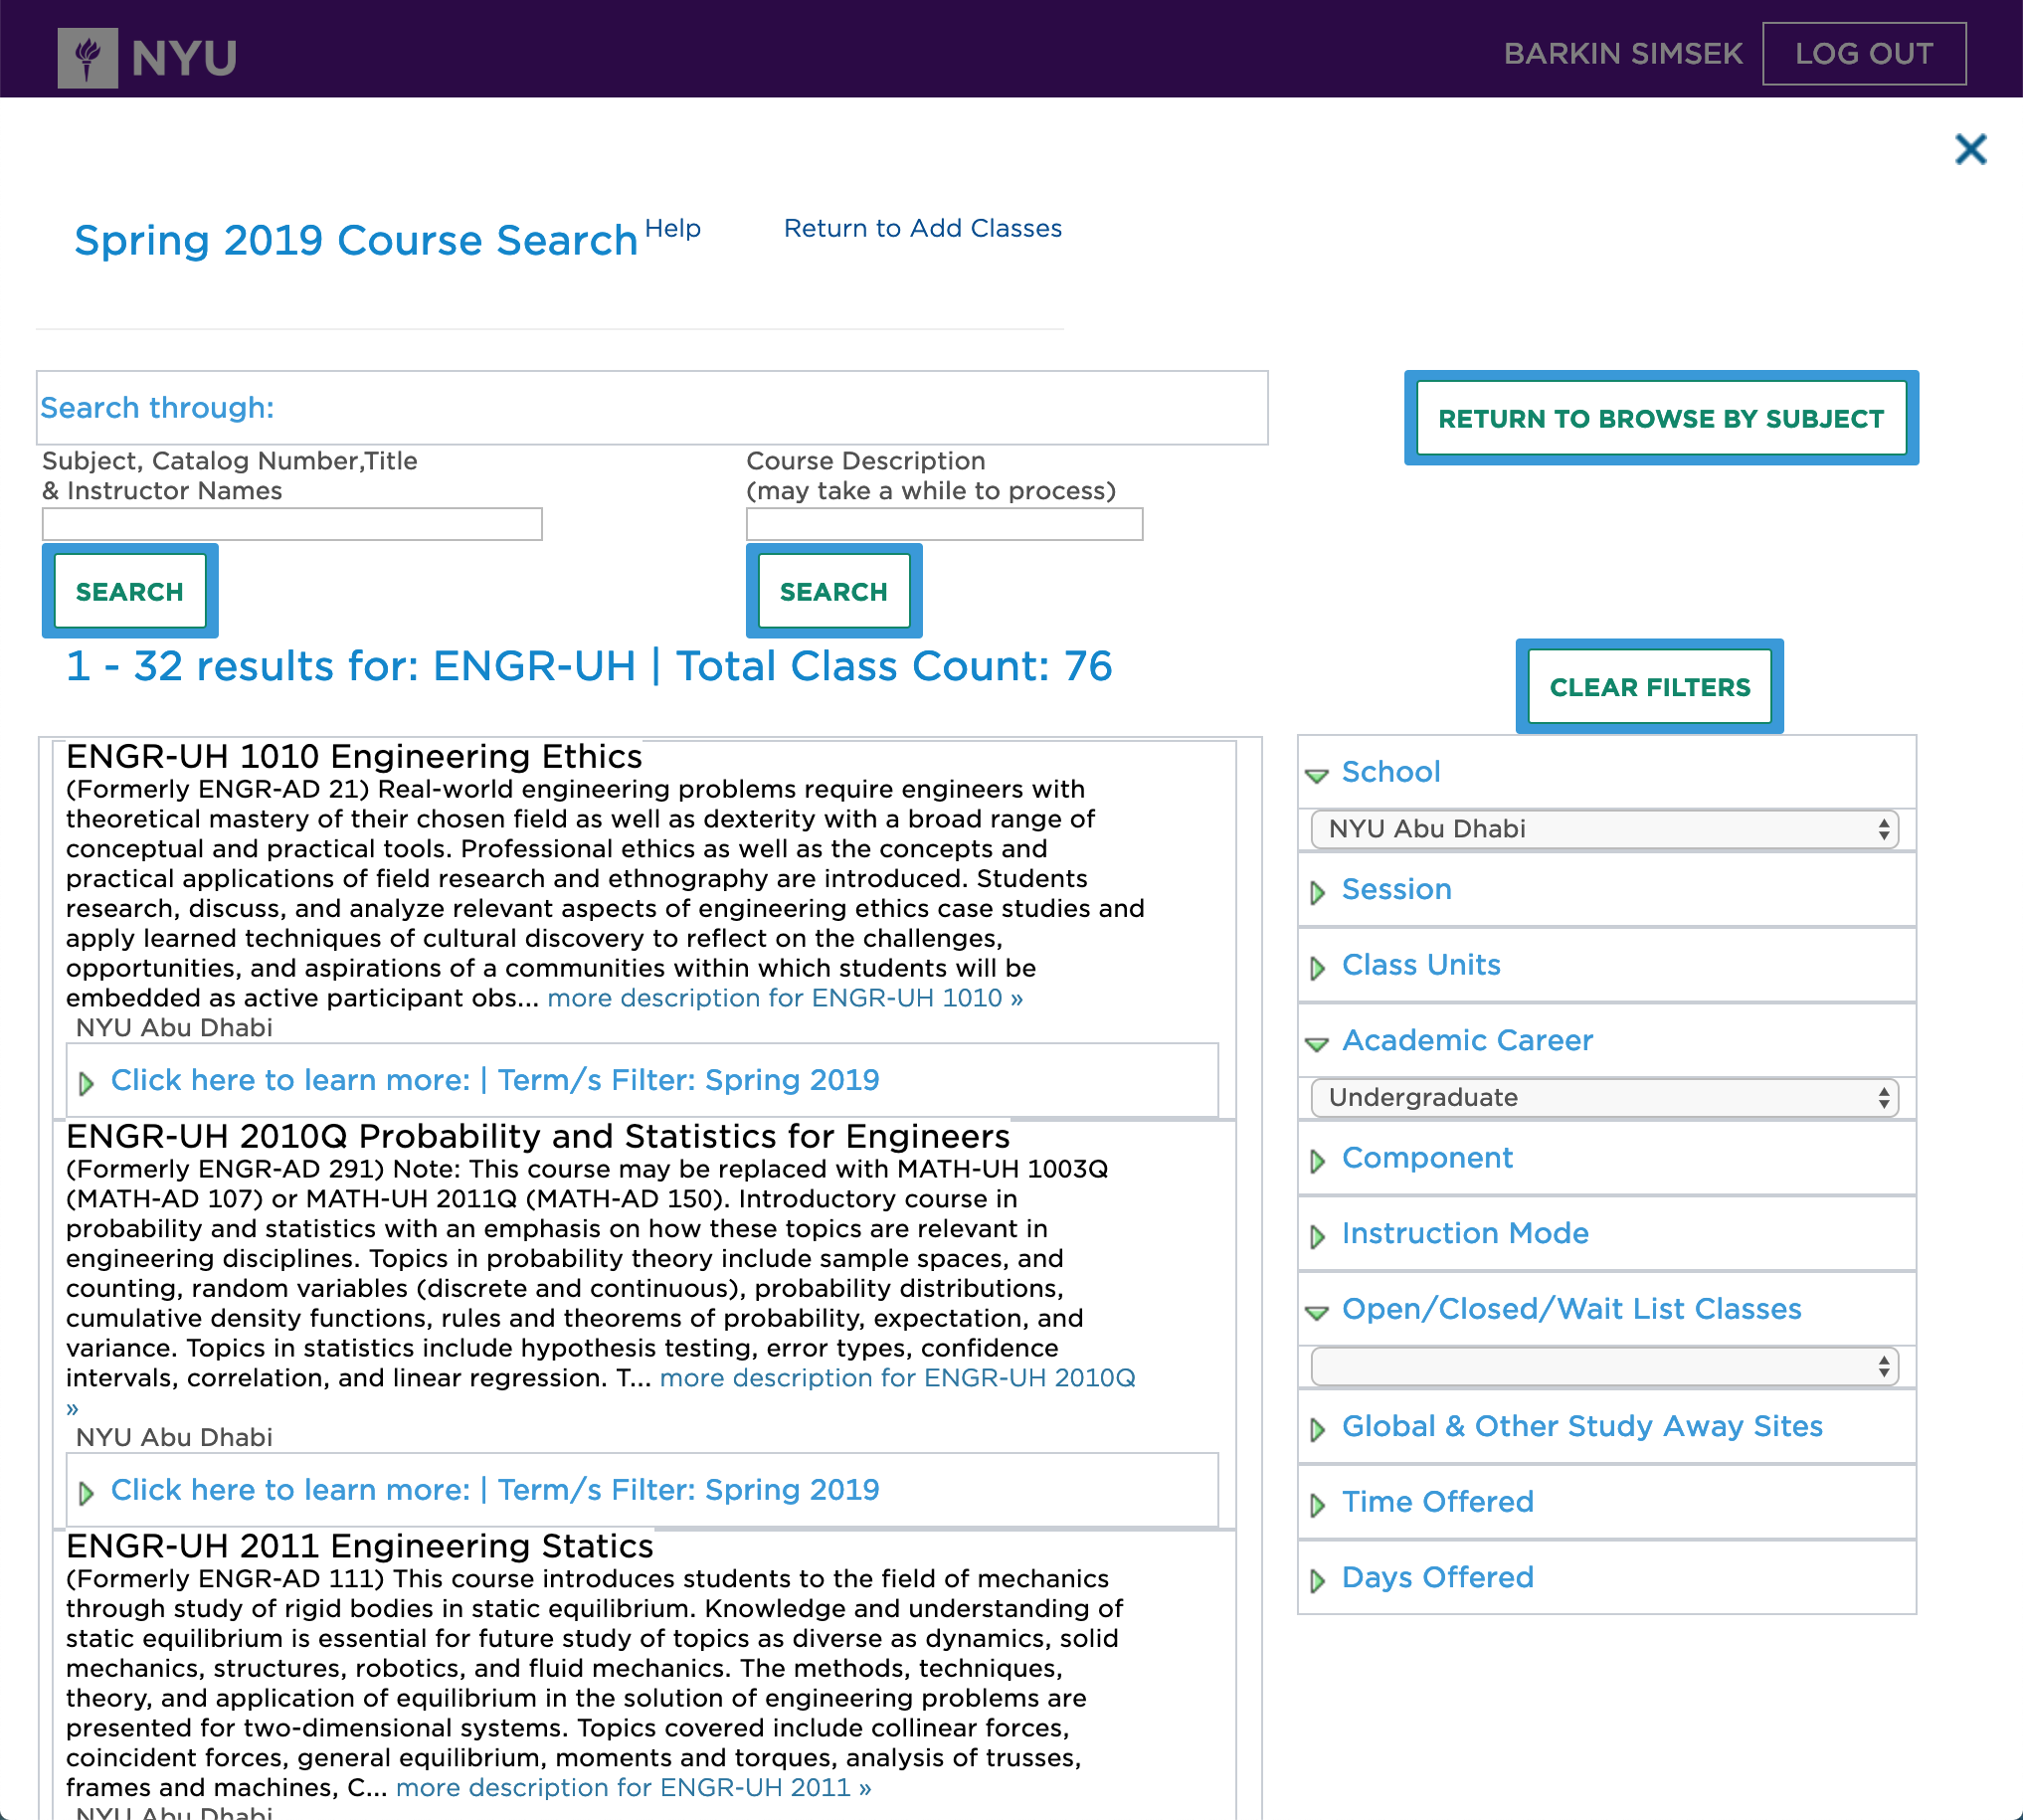
\includegraphics[width=\columnwidth]{images/6.png}
    \captionof{figure}{Course times are hidden under the Read More tab}
    \label{fig:first}
    \medskip
\endgroup

\begingroup
    \medskip
    \centering
    %width=\columnwidth
    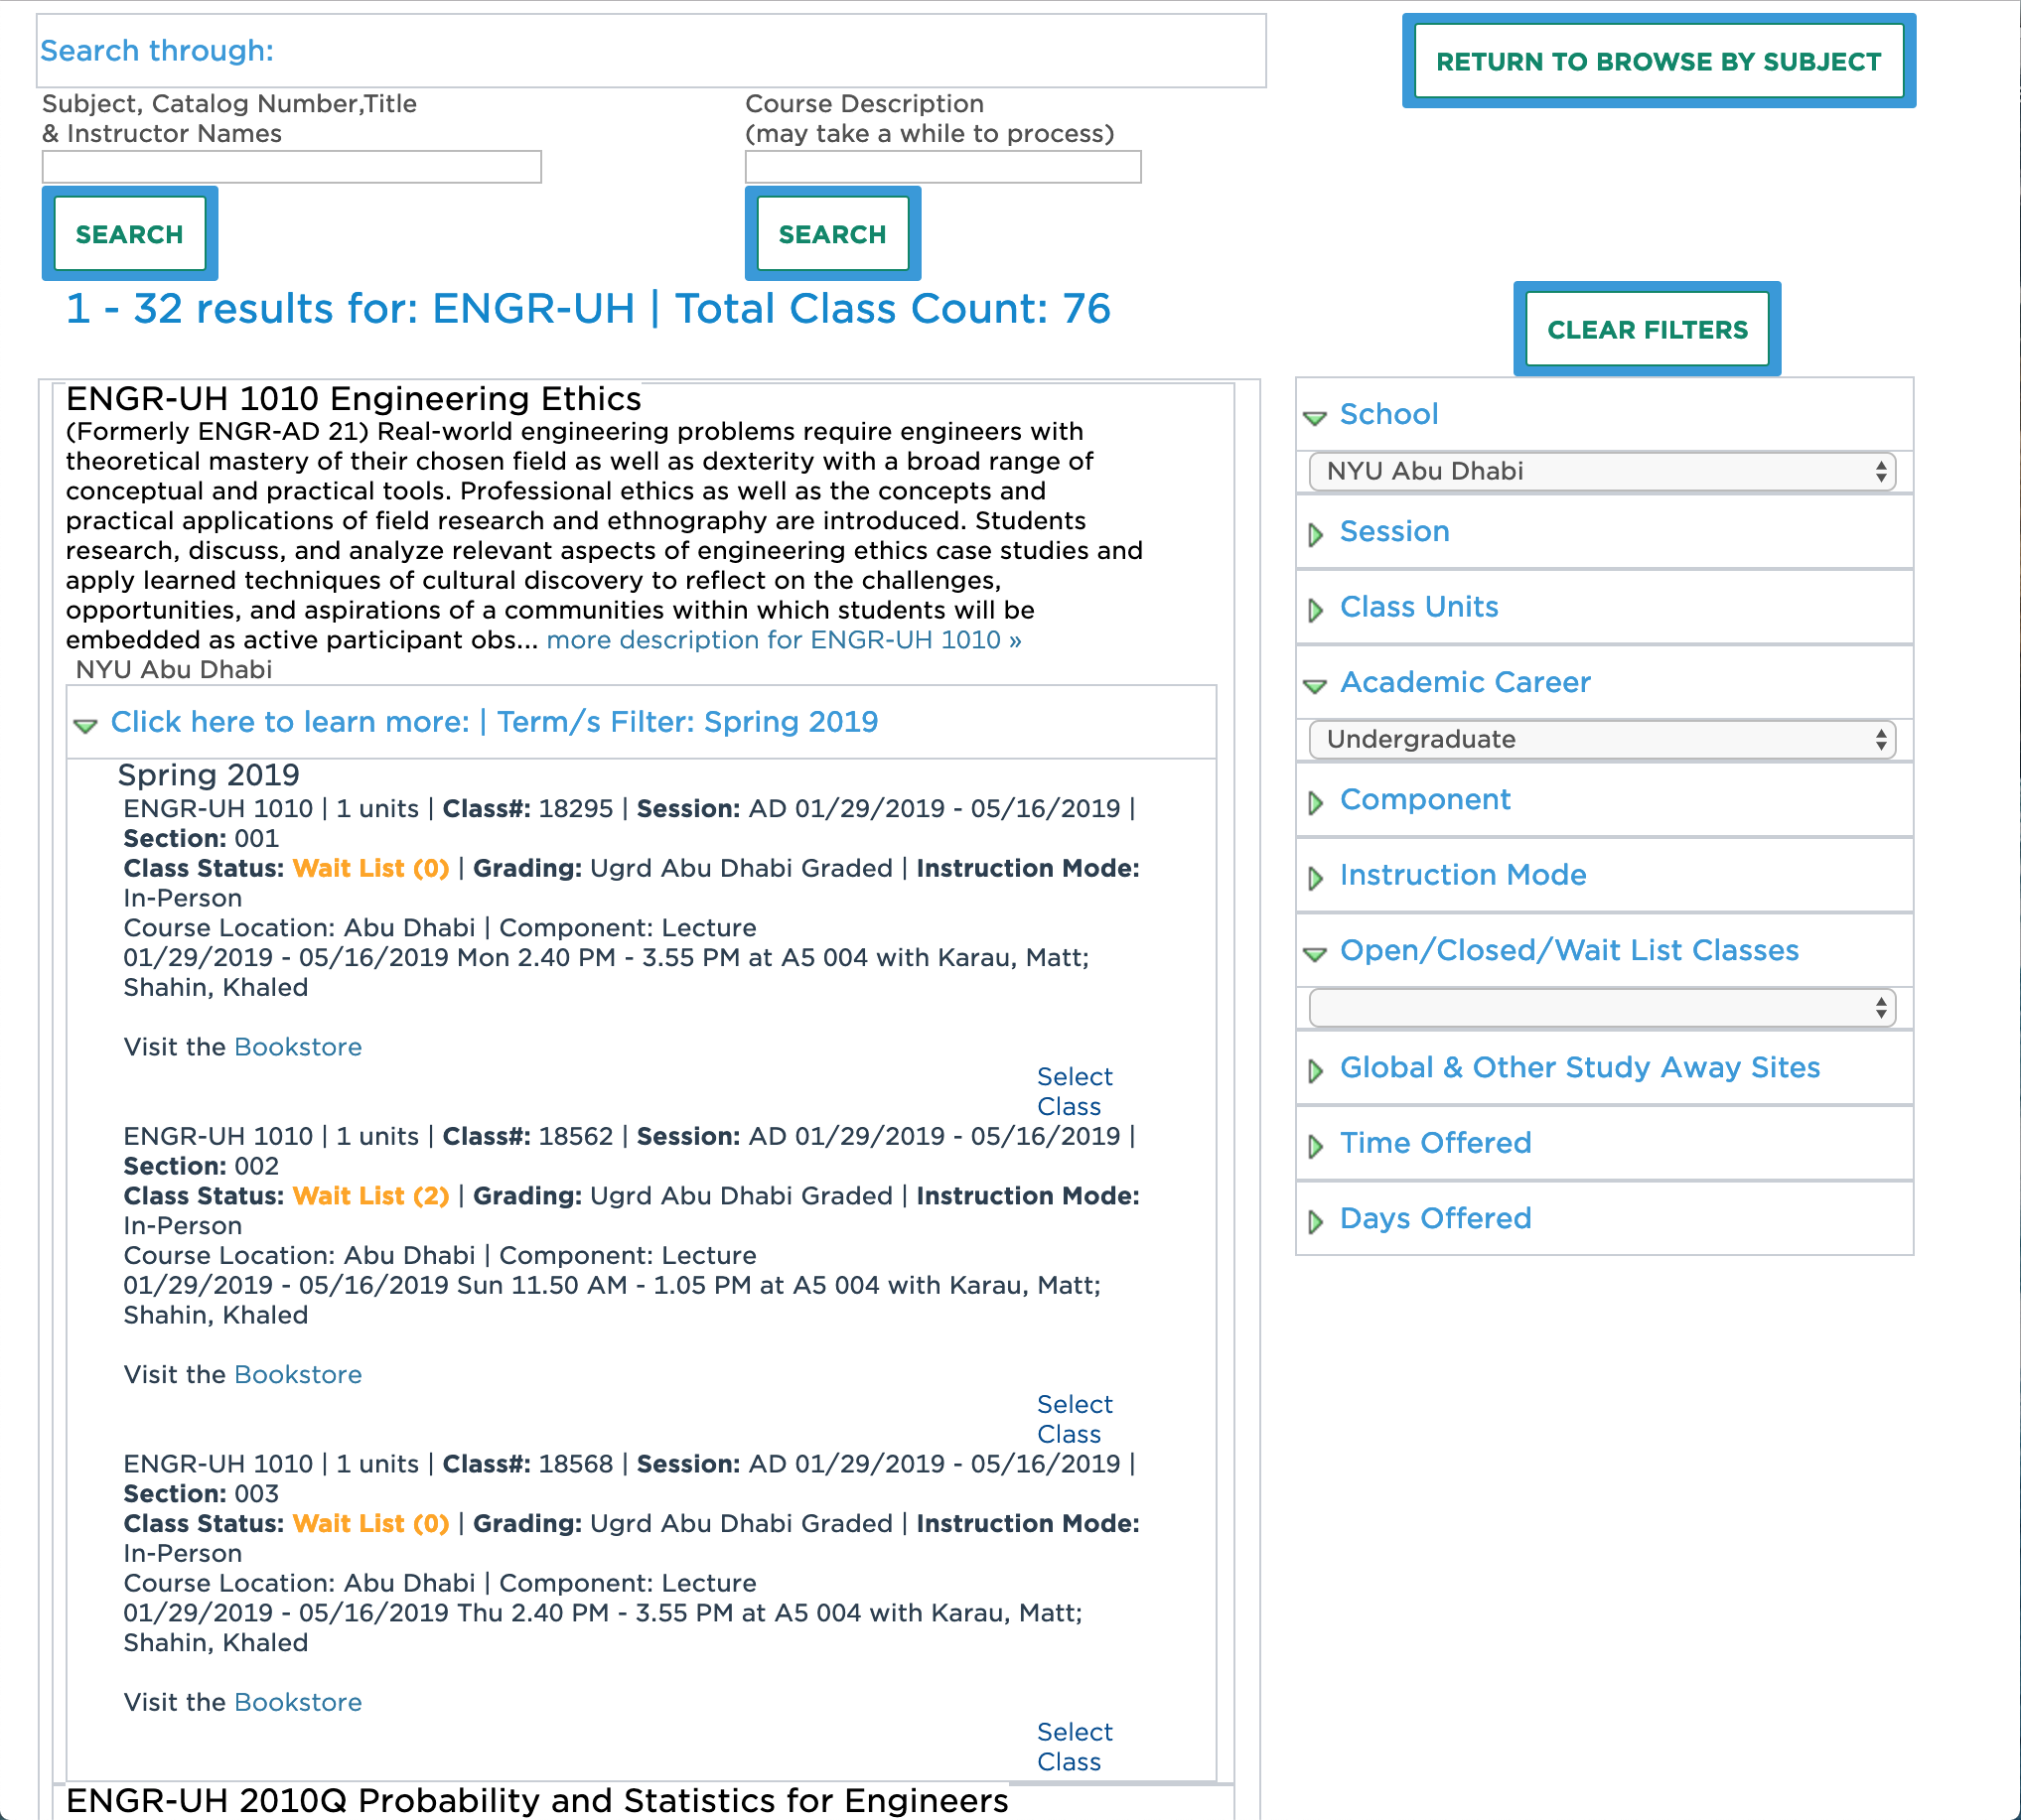
\includegraphics[width=\columnwidth]{images/7.png}
    \captionof{figure}{Course times are not emphasized nor easy to read}
    \label{fig:first}
    \medskip
\endgroup

\subsection{Summary of Solution}
An intuitive, graphical system which allows students to input their major, completed courses, and time preferences to receive a list of possible courses, a block scheduling interface, and recommended courses. This will allow students to visualize their calendar as its built to avoid conflicts.


%Architecture

%>> Abstract level
%>> Code structure

%Design Criteria

%Technologies used

\section{CONSTRAINTS}

\subsection{Data Constraints}

\noindent As the course scheduling software is heavily dependent on time and term data, one of the largest constraints stems from the source of data. For initial testing, we looked towards the NYUAD Student Portal to obtain all the data in XML format (http://services.nyuad.nyu.edu/academics/courses). The XML data was uploaded to a MySQL database, which was then accessed using a SQL database connector library in Python. Data between various tables was correlated using primary and foreign keys already provided in the XML file (see Figure \ref{fig:third}).

\begingroup
    \medskip
    \centering
    %width=\columnwidth
    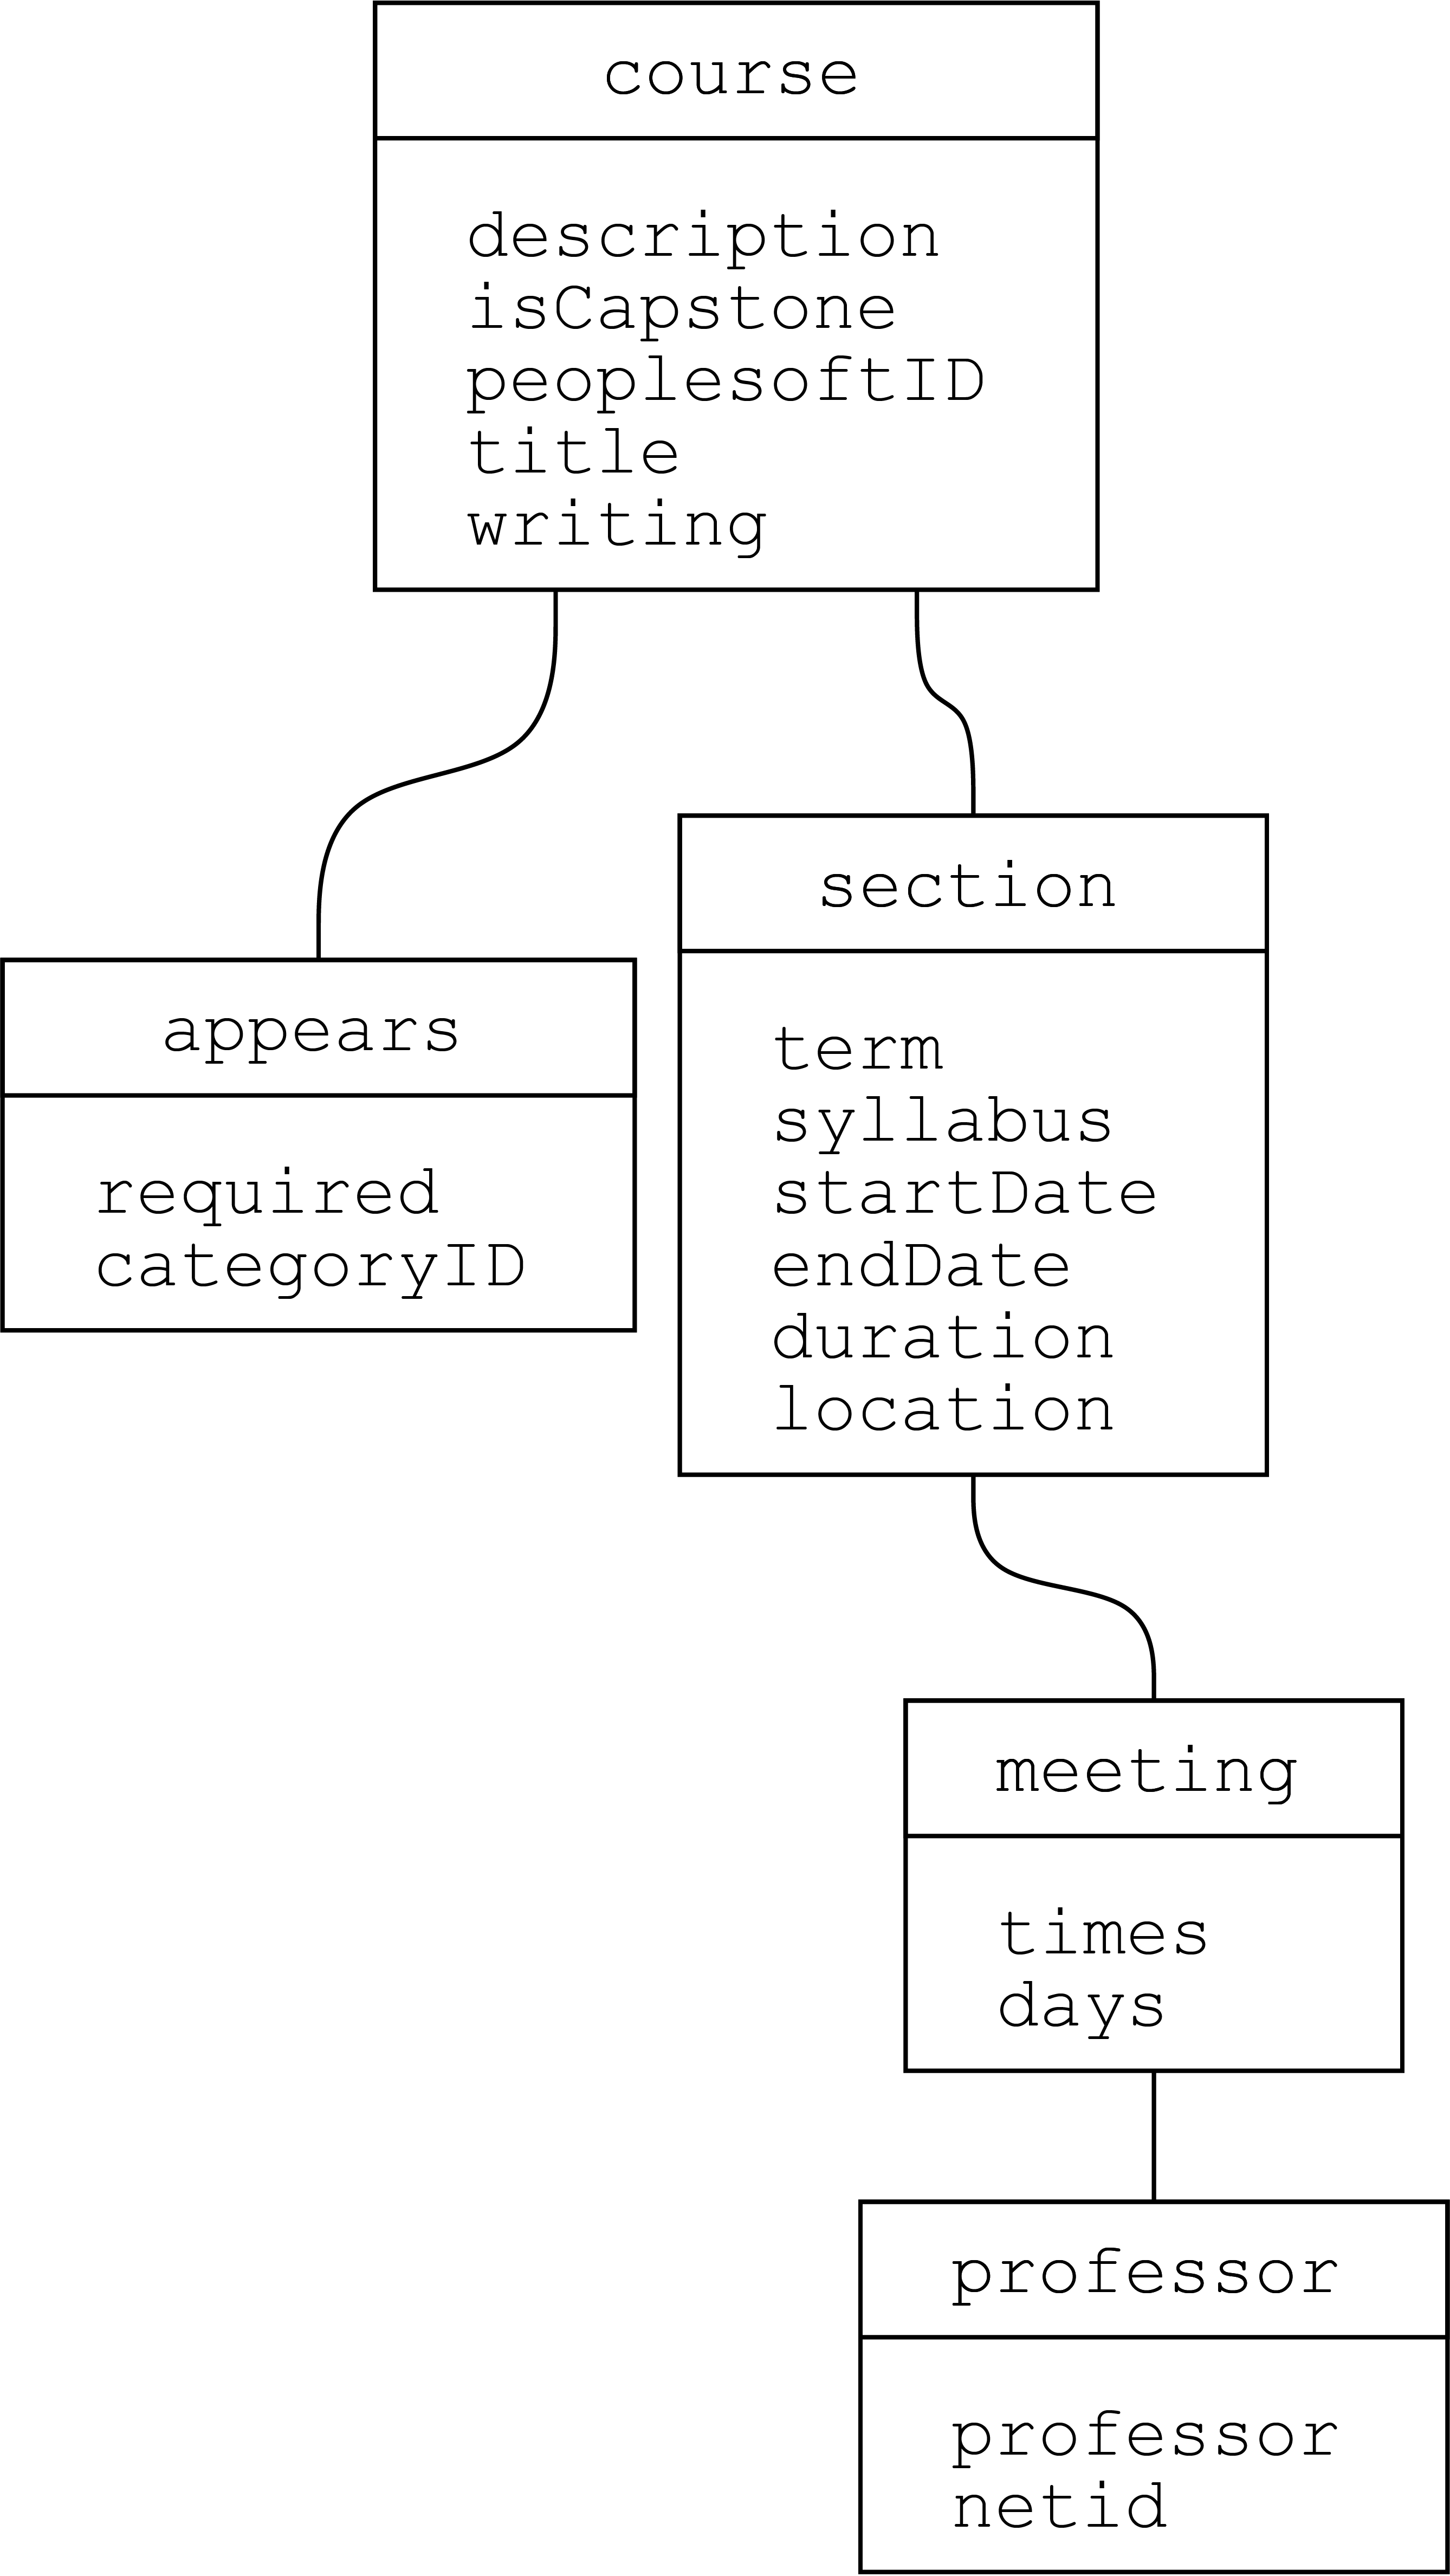
\includegraphics[scale=0.35]{images/er-diagram.png}
    \captionof{figure}{Visualization of the relational database}
    \label{fig:third}
    \medskip
\endgroup

\noindent The data constraint lies in the fact that the Student Portal's database of course information is not properly formatted; the class times are especially unorganized, with some times, for example, written in 24 hour format and others in 12 hour format. Looking towards Coursicle, a generalized scheduling app, and NYU Albert's public page, we sought to find a better source of course information; however, it seems that both services grab data from an inaccessible database. Thus, it seems that the project will be utilizing the XML file obtained from NYUAD's student portal.

\subsection{Architectural Constraints}
 \noindent As the software is meant to be part of a larger future web project, we are constrained in our architecture of the course scheduling software. Since we are avoiding the use of the PHP programming language, we are required to use a framework in which to deploy our Python script. We are considering a microframework such as Flask, which is actively maintained, allowing us a lot more freedom to write our Python script over a solution like the Django framework. 
 
 Thus, as of now, we are constrained to separating our graphical user interface (GUI) Python script (wrapped in Flask) from our back-end database interaction and information storage script (see Figure \ref{fig:first}). The idea is that the GUI script will gather presentable data from the back-end Python script and also return user selected data back to the back-end script to carry out operations.
 
\begingroup
    \medskip
    \centering
    %width=\columnwidth
    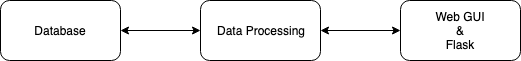
\includegraphics[width=\columnwidth]{images/high-level.png}
    \captionof{figure}{High-level model of the course planner application}
    \label{fig:second}
    \medskip
\endgroup

\section{SYSTEM ARCHITECTURE}
\subsection{High-level Architecture}

Figure \ref{fig:second} shows the high-level architecture of the course scheduling app. In summary, the user will request to create a schedule, select their (intended) major from a list of available majors and select their year, select completed requirements, and select course and time preferences. This will land the user on a scheduling page providing them with a list of recommended classes, a reminder of classes they have already taken, and also a reminder of classes that are recommended by the bulletin (based on the current semester) 

\begingroup
    \medskip
    \centering
    %width=\columnwidth
    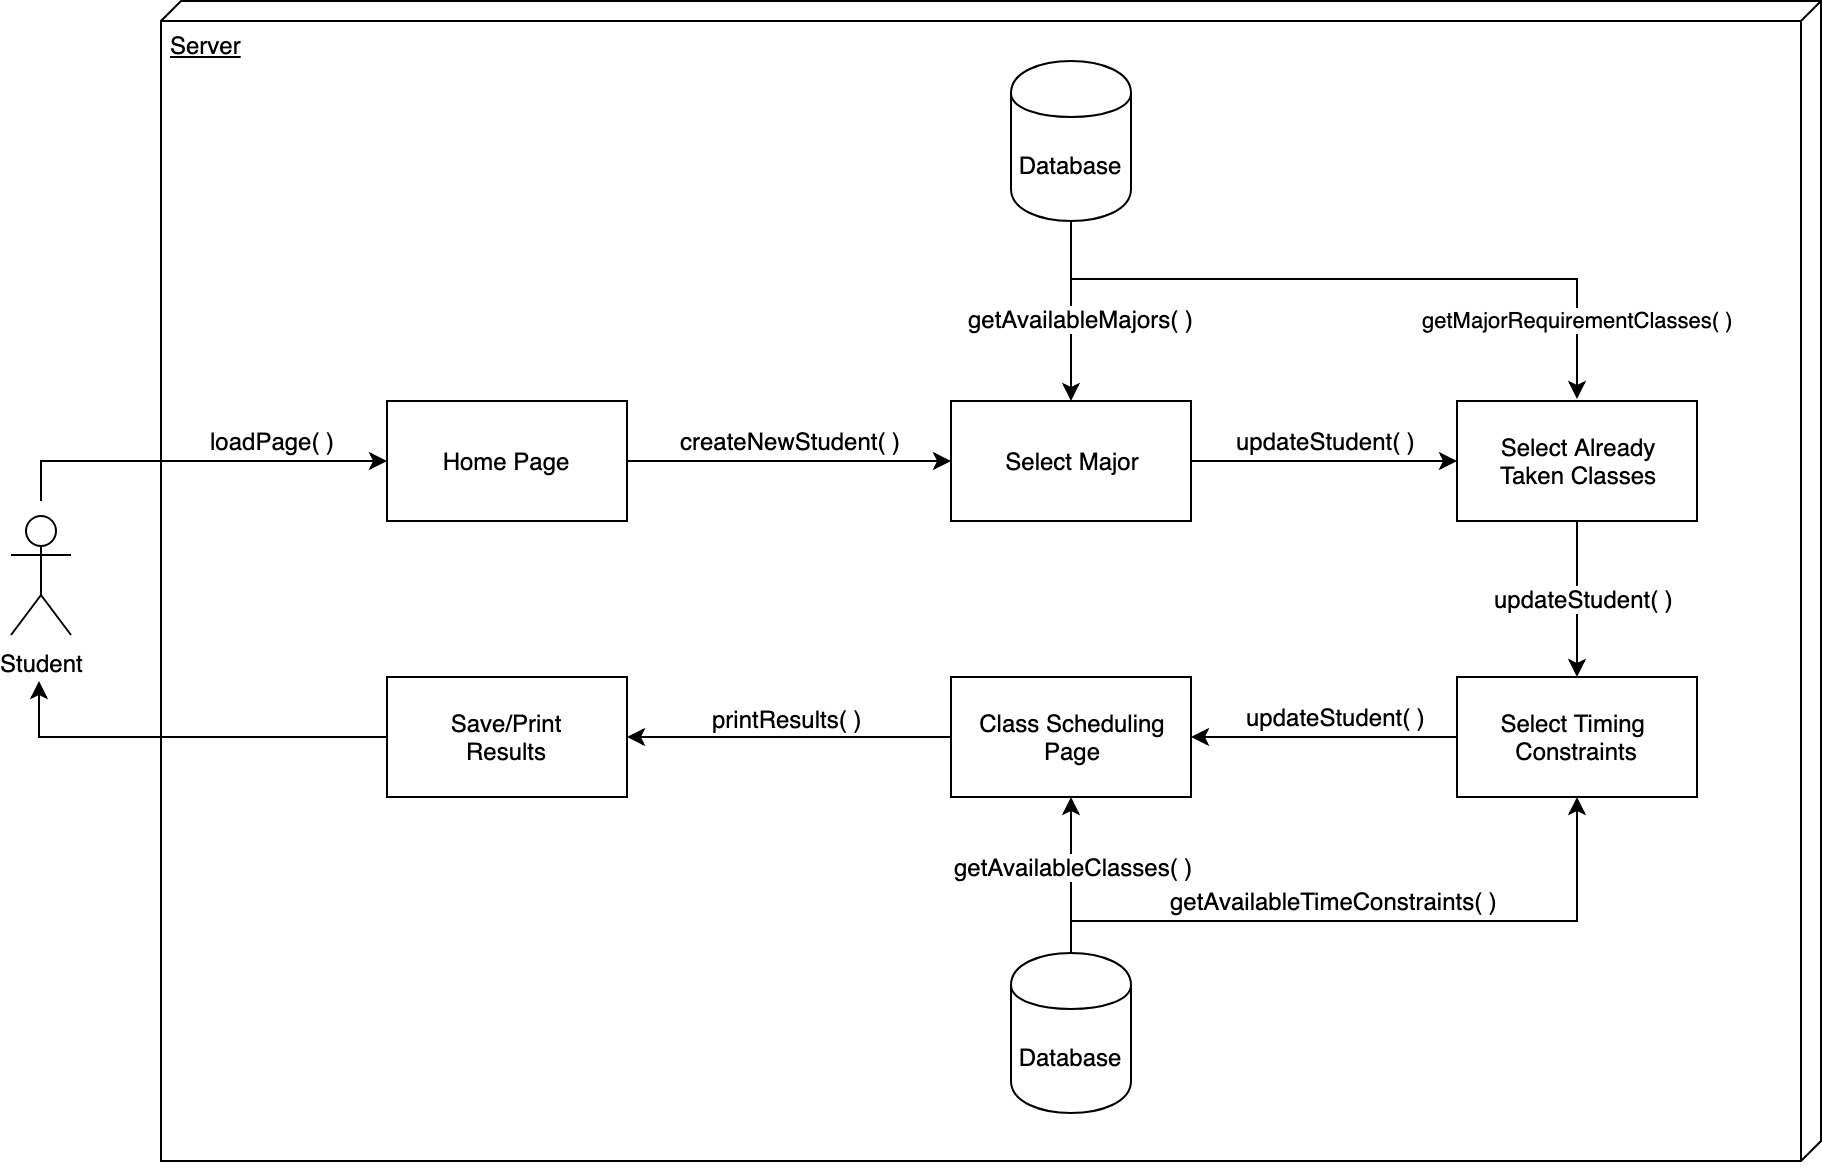
\includegraphics[width=\columnwidth]{images/full-system.png}
    \captionof{figure}{High-level model of the course planner application}
    \label{fig:second}
    \medskip
\endgroup

\subsection{Implemented Classes}
As the Python script for the GUI is wrapped in Flask, the two back-end classes will be imported into the main script and objects from both classes will be instantiated as needed. Figure \ref{fig:fourth} provides a summary of the two classes and their functionalities. Essentially, the Database class exists to interact with the mySQL database and return arrays of information. On the other hand, the Student class exists to store the information of the user and build their profile as they move through the program, all the while interacting with the Database class to obtainn information. The front-end script calls functions from both classes as needed.

\begingroup
    \medskip
    \centering
    %width=\columnwidth
    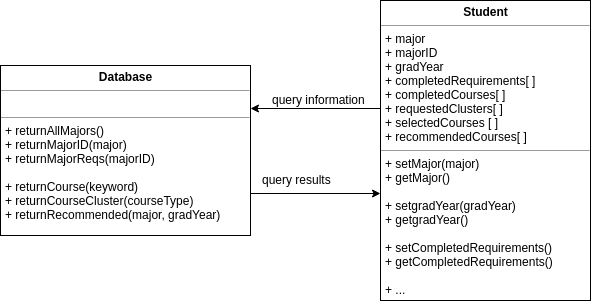
\includegraphics[width=\columnwidth]{images/classEntity.png}
    \captionof{figure}{Back-end class implementations}
    \label{fig:fourth}
    \medskip
\endgroup


\subsection{Technologies}
The system will be written in Python and Flask will be used as the web framework for deploying the application to the web server. The course information obtained from the student portal is stored in a relational MySQL database on the Linux web server. HTTP requests coming from users are handled by the Apache web server and automatically transferred to the Python App container created on the Linux web server. Later, Flask web framework takes over the requests and lets us process requests by using Python. Classes implemented in Python are used like libraries to abstract database transactions. Data that need to be transferred are being passed to classes and later classes deliver data to required destinations at a lower level.

Utilizing Flask and the Linux web server gives us the ability to deliver content to students whenever they want and wherever they are, as long as they have internet connection.

\begingroup
    \medskip
    \centering
    %width=\columnwidth
    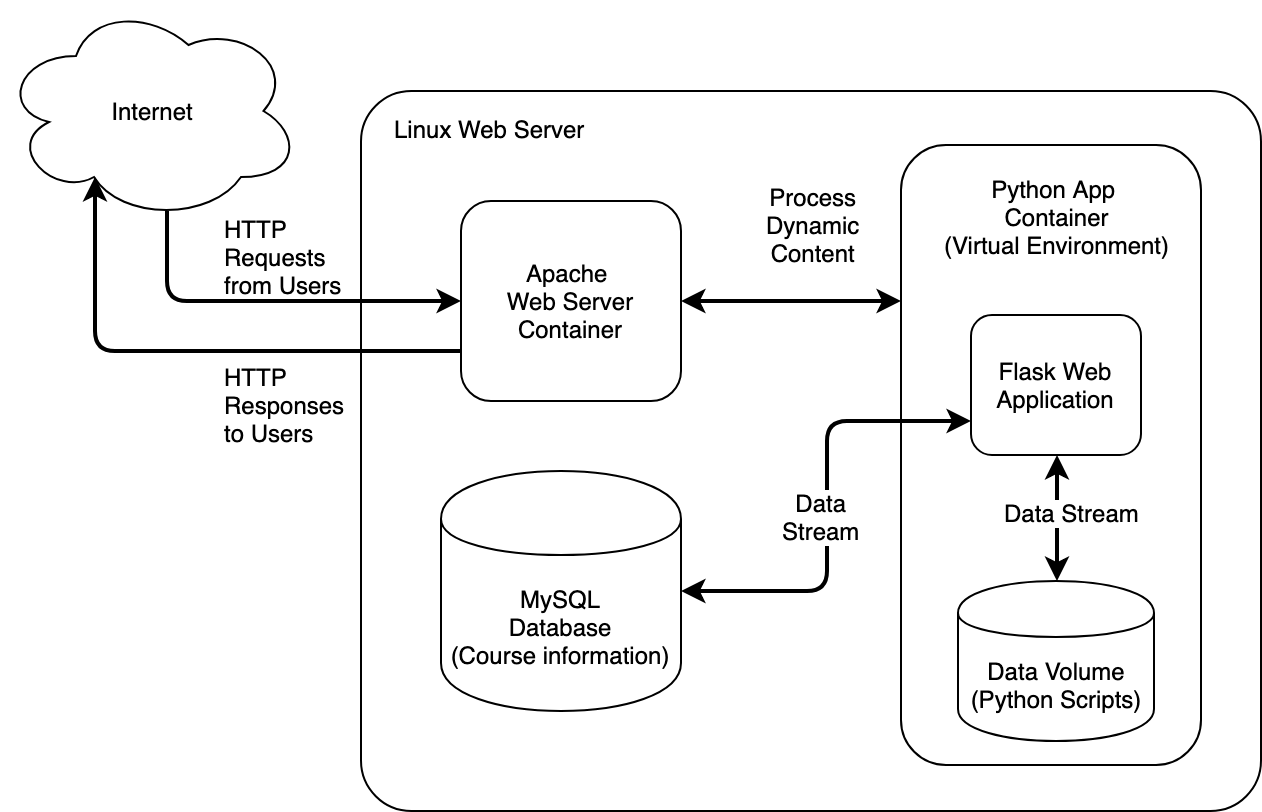
\includegraphics[width=\columnwidth]{images/detailed-high-level-diagram.png}
    \captionof{figure}{A broad summary of the technologies used}
    \label{fig:second}
    \medskip
\endgroup

\section{FUTURE PLANS}

\subsection{Milestone}
\noindent Our goal for the upcoming milestone is being able to through the background data acquisition part. We plan to successfully show the classes that a user can take. We hope to finish the visualization part but our priority is completing rough functionality. So, users will be able to enter their majors, select previously taken classes, enter various class scheduling constraints and view the list of classes that satisfy the entered criteria when the milestone is achieved.

\subsection{Future Goals}
\noindent The course scheduling software is meant to be part of a larger project called nyuad.app, which is meant to act as a more focused and accessible student portal. Our goal is to provide the course scheduling software as a service that is part of the nyuad.app project. Thus, we would like to improve on the CSS aspect of the application, making it compatible across all browsers. Another goal is to eventually conduct student feedback surveys to understand what functionality is missing or what would improve the aesthetics of the application. 


%\cite[]{datasheet}

\printbibliography



\end{document}
